\documentclass[runningheads]{llncs}

\usepackage[T1]{fontenc}
\usepackage{graphicx}
\usepackage{amsmath,amssymb}
\usepackage{booktabs}
\usepackage{multirow}
\usepackage{algorithm}
\usepackage{algorithmic}
\usepackage{hyperref}
\usepackage{xcolor}
\usepackage[fontset=fandol]{ctex}

\newcommand{\ie}{\textit{i.e.}}
\newcommand{\eg}{\textit{e.g.}}

\begin{document}

\title{可测量才可调控：博弈论共识框架\\对LLM评审团羊群效应的诊断与干预}

\titlerunning{可测量才可调控：LLM评审团的诊断与干预}

\author{Tiancheng Ma\inst{1}}
\authorrunning{T. Ma}

\institute{School of Computer Science\\
\email{author@university.edu}}

\maketitle

\begin{abstract}
多智能体大语言模型（LLM）系统通过输出聚合形成集体判断，但此类评审团是否表现出人类委员会中早有记录的羊群效应病理，以及若存在、哪类机制能够修复，目前仍缺乏深入理解。回答这两个问题需要两件仪器：测量集体行为的手段与干预集体行为的手段。本文表明，此前开发的博弈论共识框架恰好提供了这两件仪器：其 AEIC（假设-证据-推论-结论）分解通过显式结论字段使羊群效应成为可测量的量，其三层 Stackelberg 机制恰好映射到三个干预位置——聚合时校准、讨论时调控、逐实例协议路由。我们将框架置于"诊断后干预"的验证范式下，以自动化学术评审这一共识质量本质上关乎行为健康的领域为试验场。\textbf{研究一}对 300 篇分层采样的 ICLR~2024 论文进行诊断，每篇论文由 5 个同质 LLM 评审智能体组成的评审团在三种聚合条件下评审。独立 LLM 评审表现出系统性拒稿偏置（明确接收层论文的接收率仅 14.4\%）；三轮非结构化讨论触发\emph{负向棘轮}：少数派立场以 96:0 的比例向拒稿方向翻转（二项检验 $p{=}2.5{\times}10^{-29}$；消灭率 78\%），评审团评分方差坍缩 51\%（Wilcoxon $p{=}3.9{\times}10^{-32}$），均分显著下移——而与官方决议的决策一致率从未改善（61.7\%$\to$59.7\%，不显著）。跨模型复现（DeepSeek-V3、GLM-4-Flash、DeepSeek-R1）揭示了\emph{方向相反的病态吸引子}：V3 与 R1 评审团向拒稿方向棘轮化，而 GLM 评审团向接收方向棘轮化且 94\% 的结论为骑墙表述；推理能力最强的 R1（决策一致率 67.3\%）反而遭受最大的多样性坍缩（76\%）。\textbf{研究二}将框架的三个层次分别作为针对单一病理的干预。静态校准层将决策一致率从 60\% 提升至 67\%（双臂 66.7\%/67.3\%，合并 McNemar $p{=}0.034$），明确接收层从 2\% 修复至 44\%；Stackelberg 优化器在无人工提示下自主学到恒正校准项（$\tau{=}+1.04$），证明校准是博弈均衡的内生属性，其简约软实现（隐含阈值 4.88，两臂完全一致）消除了硬阈值调参的选择噪声。该精度距人类程序委员会的委员会间一致性（约 74\%，NeurIPS 一致性实验）仅 7 个百分点。提示层面的行为调控——证据锚定的少数派坚持——基本未能撼动棘轮（消灭率 78\%$\to$71\%），但保持了决策质量；这一诚实的负结果表明话术干预无法克服由能力驱动的从众。逐论文协议路由以低 56\% 的成本匹配最优固定协议（64.7\%），将讨论降级为按需调用的资源。两项研究共同确立了 LLM 共识系统的"校准优先"原则，并表明行为健康指标——少数派存活率、方差保持、漂移——是比决策准确率敏感得多的评审团级评估终点。

\keywords{多智能体共识 \and Stackelberg博弈 \and LLM同行评审 \and 羊群效应 \and 谄媚 \and 校准聚合}
\end{abstract}

%======================================================================
\section{引言}
\label{sec:intro}
%======================================================================

由大语言模型（LLM）驱动的多智能体系统日益承担起\emph{集体判断}任务：多个模型实例独立分析问题、交换立场，并聚合为共识决策~\cite{han2024llm,tran2025multiagent,wang2023selfconsistency,du2024improving}。然而，对此类系统的评估至今仍是一维的：只看最终决策的准确率。评审团\emph{如何}抵达决策——它是否保留了正当的异议、维持了评分多样性、是否基于正确的理由收敛——却很少被测量，因为自由文本形式的审议使这些行为量难以提取。

这种忽视是危险的。人类委员会存在羊群效应是众所周知的：评审人之间的讨论与分数压缩和从众效应相关，初始多数派立场会不成比例地决定最终结果。LLM 评审团是否表现出类似的病理——其方向和量级如何——在很大程度上尚未得到刻画。这一问题对机制设计至关重要：若羊群效应确实存在，其结构决定了哪一类干预能够修复它。如果病理是静态偏置，聚合时校正即可；如果讨论本身摧毁信息，则需要行为调控；如果审议只在部分实例上有所回报，那么路由才是合适的方案。

回答上述任何一个问题都需要传统管道所缺乏的仪器：羊群效应必须先变得\emph{可测量}，才能被治疗。本文表明，此前开发的博弈论共识框架恰好提供了这些仪器。其 \textbf{AEIC 分解}（第~\ref{sec:aeic}~节）将每个智能体的输出结构化为假设、证据、推论与一个显式结论字段——一枚立场探针，使集体行为可被直接测量（比非结构化文本的提取可靠性高 28 个百分点）。其\textbf{三层 Stackelberg 激励机制}（第~\ref{sec:game}~节）具有形式化的 $\epsilon$-激励相容保证（第~\ref{sec:theory}~节），恰好映射到三个干预位置：聚合时的静态参数优化、讨论中的在线与动态调控、以及逐实例的\textbf{自适应协议路由}（第~\ref{sec:topology}~节）。在问答基准上，框架已回答了\emph{决策质量}问题（路由器实现 87.6\% 共识准确率）；本文则让它回答\emph{行为健康}问题——以自动化学术评审为试验场，这是一个高风险且本质上关乎行为的领域，LLM 智能体已在其中为研究论文生成评审意见~\cite{liang2024llmreview,jin2024agentreview}。

验证遵循\emph{诊断后干预}设计（第~\ref{sec:exp}~节）。\textbf{研究一}汇集了 300 篇分层采样的 ICLR~2024 论文（明确接收/边界/明确拒稿），由 5 个同质 LLM 评审智能体组成的评审团在三种条件下评审——独立聚合、三轮讨论与元评审综合。诊断以强有力的统计证据确认了三种病理：独立评审中的系统性\emph{拒稿偏置}（明确接收层论文接收率仅 14.4\%）；讨论中的\emph{负向棘轮}——少数派立场以 96:0 向拒稿方向翻转（$p{=}2.5{\times}10^{-29}$），消灭率 78\%，评分方差坍缩 51\%（$p{=}3.9{\times}10^{-32}$）；以及讨论完全没有带来决策收益（一致率 61.7\%$\to$59.7\%，不显著）。在 DeepSeek-V3、GLM-4-Flash 与 DeepSeek-R1 上的跨模型复现表明，羊群效应是普遍的，但其\emph{方向}依赖于模型：V3 与 R1 评审团向拒稿方向棘轮化，而 GLM 评审团向接收方向棘轮化；且推理能力最强的 R1 遭受最大的多样性坍缩（76\%）——能力并不能抵御羊群效应。

\textbf{研究二}随后将框架的三个层次部署为针对性干预，每层对应一种病理。静态层（\emph{软校准聚合}）将决策一致率从 60\% 提升至 67\%（双臂 66.7\%/67.3\%，合并 McNemar $p{=}0.034$），明确接收层从 2\% 修复至 44\%，隐含阈值 4.88 跨臂完全一致；Stackelberg 优化器自主学到恒正校准项（$\tau{=}+1.04$），证明校准是均衡的内生属性。该精度距人类程序委员会的委员会间一致性（约 74\%，NeurIPS 一致性实验）仅 7 个百分点——决议噪声构成固有测量天花板。动态层（\emph{证据锚定的行为调控}）基本未能撼动负向棘轮（消灭率 78\%$\to$71\%；被干预少数派的坚持率 29\% 对 28\%），但保持了决策质量——这一诚实的负结果表明提示层面的调控无法克服由能力驱动的从众。路由层（\emph{逐论文协议选择}）以低 56\% 的推理成本匹配最优固定协议（64.7\%），将审议确立为按需调用的资源而非常规默认。

我们的贡献如下：
\begin{enumerate}
    \item \textbf{LLM 评审团的大规模配对诊断。}以配对设计和强有力的统计证据确立三种病理——拒稿偏置、负向棘轮、多样性坍缩；所采用的行为健康指标（少数派存活、方差保持、漂移）被证明远比决策准确率敏感。
    \item \textbf{具有相反病态吸引子的跨模型普遍性。}羊群效应的方向依赖于模型（拒稿棘轮 vs. 接收谄媚），且更强的推理能力与更强的多样性坍缩共现。
    \item \textbf{校准优先的干预原则。}聚合时校准修复决策偏置（+6~7 个百分点）并逼近人类委员会间一致性定义的测量天花板；提示层面的行为调控无法恢复多样性；逐论文路由在低 56\% 成本下保持准确率——三者共同描绘了哪类机制治疗哪种病理的图谱。
\end{enumerate}

%======================================================================
\section{相关工作}
\label{sec:related}
%======================================================================

\paragraph{多智能体大语言模型共识。}
对多个大语言模型（LLM）输出的聚合研究已经过几种范式的探索。自洽性（Self-consistency）~\cite{wang2023selfconsistency} 对多条推理路径进行采样，并选择频率最高的答案。多智能体辩论（Multi-agent debate）~\cite{du2024improving,choi2025debate} 将此扩展为多个模型实例之间的迭代讨论。ChatEval~\cite{chan2023chateval} 将此应用于评估任务。Zhao 等人~\cite{zhao2024electoral} 基于社会选择理论提出了基数投票机制。Li 等人~\cite{li2025dynamic} 引入了动态权重。

这些系统中的一个关键故障模式是\emph{阿谀奉承（sycophancy）}——智能体在没有进行真正推理的情况下采纳多数派立场。Bertalani\v{c} 和 Fortuna~\cite{bertalanic2026cost} 提供了迄今为止最全面的实证描述，记录了同构多智能体辩论（$n{=}10$）中的三种故障路径：谄媚的从众行为（高达 85.5% 的模式采纳）、语境脆弱性（高达 70% 原本正确的智能体被同伴的理由动摇），以及共识崩溃（多数决投票丢弃正确答案的预言机差距高达 32.3 个百分点）。他们的核心发现——没有结构化角色的同构团队无法从无指导的同伴交流中获益——直接激发了我们通过 AEIC 分解进行结构化角色强制执行，以及通过斯塔克尔伯格机制（Stackelberg mechanisms）进行行为规范的工作。Liu 等人~\cite{liu2025memorycurse} 进一步表明，扩展的智能体内存在博弈论设置中可能会\emph{降低}合作水平，在 28 种模型-博弈配置中，有 18 种更长的回忆会减少合作意图——这一发现与我们的结果一致，即即使智能体可以访问差异化信息，质量信号也无法可靠地区分正确和误导性的知识。

Pitre 等人~\cite{pitre2025consensagent} 通过 ConsensAgent 解决了阿谀奉承问题，该机制根据智能体交互动态微调提示以减轻羊群效应。ConsensAgent 在单一辩论拓扑内的提示层面上运行。我们的动态调节有根本的不同：我们不为单个智能体优化提示，而是监控跨轮次的\emph{集体行为动态}（立场变化率、多数比率、收敛速度），并针对检测到的特定病理特征（阿谀奉承与僵局）应用差异化干预——参数调整\emph{和}提示修改。Swamy 等人~\cite{swamy2025peacemaker} 为多智能体辩论中的阿谀奉承提供了正式指标；他们关于阿谀奉承水平在不同智能体角色中存在显著差异的发现，为我们基于立场变化的检测提供了依据。最近，Kumarappan 等人~\cite{kumarappan2026alignment} 证明，多智能体的阿谀奉承是结构性的（存在于基础模型中，而不仅仅是基于人类反馈的强化学习（RLHF）工件），缓解措施应该在“管道层面针对结构化异议”进行——这正是我们的斯塔克尔伯格动态调节通过行为状态检测和自适应 EV 权重抑制所实现的。

\paragraph{结构化推理分解。}
思维链（Chain-of-Thought）提示~\cite{wei2022chain} 引发逐步推理，思维树（Tree-of-Thoughts）~\cite{yao2024tree} 将此扩展到推理路径的结构化探索。ReAct~\cite{yao2023react} 交错进行推理与行动。这些方法对推理进行分解以提高\emph{个体}答案的质量。我们的 AEIC 分解服务于不同的目的：它将智能体的输出结构化为四个可解析的字段（假设、证据、推论、结论），以实现\emph{跨智能体}的操作——从明确的结论（Conclusion）字段进行可靠的立场提取（比非结构化提取高出 28 个百分点）、用于自适应路由的跨拓扑投票模式比较，以及用于动态调节机制的群体级行为动态监控（见第 \ref{sec:dynamic} 节）。该分解并非旨在改进每个智能体的推理；其设计目的是使集体行为具有可观察性和可调节性。

\paragraph{多智能体系统中的通信拓扑。}
通信结构对多智能体性能的影响已在多种语境中进行了探讨。Chen 等人~\cite{chen2023agentverse} 使用了集中式评估器（星型拓扑）。顺序架构出现在智能体链（chain-of-agents）设计中~\cite{hong2023metagpt}。Du 等人~\cite{du2024improving} 研究了辩论拓扑（完全图）。Chen 等人~\cite{chen2024reconcile} 在不同的大语言模型中引入了带有置信度加权投票的圆桌会议。最近，RUMAD~\cite{wang2026rumad} 应用强化学习在单一拓扑类型内自适应地控制辩论轮次和智能体选择。我们的方法在三个方面有所不同：我们在五种根本不同的通信结构（并行、顺序、星型、辩论、分层）中进行选择，使用可解释的投票模式特征而不是不透明的 RL 策略，并将我们的机制建立在博弈论的激励兼容性保证上。

\paragraph{多智能体系统中的内存。}
近期的几项工作研究了智能体内存在如何影响多智能体动态。EquiMem~\cite{meng2026equimem} 将多智能体辩论中的共享内存公式化为一种零信任内存博弈，其中均衡状态校准了最佳的内存信任度——这与我们的博弈论方法类似，但侧重于内存完整性而非共识激励。Liu 等人~\cite{liu2025memorycurse} 证明了一种矛盾的“内存诅咒”，即在基于大语言模型的社会困境中，扩大回忆能力会降低合作意图（在 28 个模型-博弈配置中有 18 个出现此情况），这表明更多的历史信息并不能提高集体决策质量。这补充了我们的发现（第 \ref{sec:exp} 节），即源自 AEIC 结构的质量信号无法区分正确与误导性的知识：这两个结果都表明，当智能体共享同一个底层大语言模型时，更丰富的个人信息——无论是历史内存还是质量得分——都不一定会改善共识。我们的动态调节机制（第 \ref{sec:dynamic} 节）通过对可观察的集体行为进行操作，而不是根据每个智能体的质量或内存内容进行操作，从而解决了这个问题，这使得它对信号限制和内存质量变化都具有鲁棒性。

\paragraph{博弈论与大语言模型。}
Sun 等人~\cite{sun2025gametheory} 提供了大语言模型应用的博弈论分类体系。Yi 等人~\cite{yi2025debate} 将多智能体辩论建模为具有纳什均衡的贝叶斯博弈。Rauba 等人~\cite{rauba2025principal} 主张对大语言模型系统进行委托-代理（principal-agent）建模。Liu 等人~\cite{liu2025interpretable} 使用大语言模型进行自动机制设计。最近，Meng 等人~\cite{meng2026equimem} 将多智能体辩论中的共享内存构建为一个零信任内存博弈，在该博弈中，均衡会校准最佳的内存信任度，而不假设智能体是诚实的；Anand 等人~\cite{anand2026resilient} 将大语言模型智能体协议定为一个拜占庭共识博弈，证明了受提示引导的智能体在经典理论保证收敛的地方无法达成一致。我们的斯塔克尔伯格（Stackelberg）公式与同时移动均衡和拜占庭共识方法不同，它将机制设计者建模为一个领导者，他在智能体行动之前\emph{承诺}采用某种聚合规则——这非常适合于旨在通过可信的承诺来塑造追随者行为的机制设计，并且与智能体诚实假设或容错保证无关。

\paragraph{分布式系统中的斯塔克尔伯格博弈。}
斯塔克尔伯格激励机制在联邦学习（federated learning）~\cite{fu2024stackelberg,guo2023incentive}和众包（crowdsourcing）~\cite{wang2024incentive}中已建立。Saig 等人~\cite{saig2024incentivizing} 应用契约理论（contract theory）来激励大语言模型生成高质量的文本。Xu 等人~\cite{xu2026rcbsf} 将斯塔克尔伯格博弈应用于多智能体合同修订。据我们所知，先前没有任何工作将斯塔克尔伯格机制设计应用于带有自适应拓扑路由的多智能体大语言模型共识。

\paragraph{与最相关工作的定位。}
表~\ref{tab:related} 将我们的框架与四个最相关的方法进行了对比。

\begin{table}[t]
\caption{与最相关工作的比较。}\label{tab:related}
\centering\small
\begin{tabular}{@{}lccccc@{}}
\toprule
& \makebox[1.8cm]{\shortstack{正式\\激励}} & \makebox[1.6cm]{\shortstack{拓扑\\选择}} & \makebox[1.6cm]{\shortstack{阿谀奉承\\解决方案}} & \makebox[1.5cm]{\shortstack{结构化\\输出}} & \makebox[1.5cm]{\shortstack{行为\\规范}} \\
\midrule
标准辩论（Standard Debate）~\cite{du2024improving} & --- & --- & --- & --- & --- \\
ConsensAgent~\cite{pitre2025consensagent} & --- & --- & 提示层级 & --- & --- \\
RUMAD~\cite{wang2026rumad} & --- & \checkmark$^\dagger$ & --- & --- & --- \\
Bertalani\v{c} 等人~\cite{bertalanic2026cost} & --- & --- & 仅限分析 & --- & --- \\
\midrule
\textbf{本项研究} & \checkmark$^\ddagger$ & \checkmark & \checkmark & \checkmark & \checkmark \\
\bottomrule
\end{tabular}
\\[2pt]
{\footnotesize $^\dagger$仅限拓扑内部（改变辩论轮次/参与度）。$^\ddagger$斯塔克尔伯格 $\epsilon$-激励兼容性（定理~\ref{thm:ic}）。}
\end{table}
%======================================================================
\section{AEIC分解与质量信号}
\label{sec:aeic}
%======================================================================

我们引入了 AEIC 分解，这是一种结构化推理协议，可在不同通信拓扑结构中实现可靠的结论提取。从 AEIC 组件导出的质量信号同时用作斯塔克尔伯格机制设计的形式化接口（第 \ref{sec:game} 节）。

\subsection{结构化推理分解}

给定一个问题 $x$，每个智能体 $i \in \{1, \ldots, n\}$ 生成一个结构化响应，将其分解为四个组件：

\begin{itemize}
    \item \textbf{假设 (A)}：智能体采纳的前提或假说。
    \item \textbf{证据 (E)}：支持其分析的事实主张列表：$E_i = \{e_{i,1}, \ldots, e_{i,k_i}\}$。
    \item \textbf{推理 (I)}：将证据与结论连接起来的推理链。
    \item \textbf{结论 (C)}：附有理由的最终答案。
\end{itemize}

这种分解通过提示工程（prompt engineering）来强制执行，并服务于两个目的：(1)~将智能体输出结构化为可解析的组件，从而在所有通信拓扑中实现可靠的结论提取和一致的立场识别——这是其主要经验价值（第 \ref{sec:exp} 节）；(2)~它提供了可分离的组件，借此计算质量信号，充当斯塔克尔伯格机制设计的形式化接口（第 \ref{sec:game} 节），尽管实验表明，当智能体共享同一底层大语言模型（LLM backend）时，这些信号的判别能力有限（第 \ref{sec:exp} 节）。

\subsection{四维质量信号}

根据每个智能体的 AEIC 输出，我们利用基于嵌入相似性的方法计算四个质量信号：

\begin{definition}[质量信号]
令 $\mathrm{sim}(\cdot, \cdot)$ 表示句子嵌入空间中的余弦相似度。对于智能体 $i$：
\begin{align}
    \mathrm{IC}_i &= \mathrm{sim}(I_i, C_i) \\
    \mathrm{EC}_i &= \tfrac{1}{|E_i|}\textstyle\sum_{e \in E_i} \mathrm{sim}(e, C_i) \\
    \mathrm{EQ}_i &= f_{\mathrm{quality}}(E_i) \\
    \mathrm{EV}_i &= \tfrac{1}{|\mathcal{N}_i|}\textstyle\sum_{j \in \mathcal{N}_i} \mathrm{sim}(E_i, E_j)
\end{align}
其中，IC 衡量推理与结论（Inference--Conclusion）的一致性，EC 衡量证据与结论（Evidence--Conclusion）的支撑力度，EQ 评估证据质量，EV 捕捉跨智能体的证据共识。
\end{definition}

此处 $\mathcal{N}_i$ 表示通信拓扑图中智能体 $i$ 的邻居，而 $f_{\text{quality}}$ 评估证据覆盖率和具体程度。按照设计，IC、EC 和 EQ 衡量的是\emph{个体推理一致性}：智能体的分析在内部一致、支持度充分且周密的程度。EV 衡量的是\emph{跨智能体共识}：某个智能体的证据与其邻居的一致性程度。这种区别对激励设计而言很重要——因为通过阿谀奉承行为可以夸大 EV 的数值。但是，正如我们的实验所展示的（第 \ref{sec:exp} 节），当智能体共享同一底层大语言模型时，这些衡量连贯性的信号无法区分正确和错误的推理：连贯的错误答案与正确答案的得分一样高。

\subsection{智能体类型空间}
\label{sec:type}

借鉴 Saig 等人的做法~\cite{saig2024incentivizing}，我们通过一种可观察的\emph{类型}对每个智能体进行建模：

\begin{definition}[智能体类型]
针对问题 $q$，智能体 $i$ 的类型为：
\begin{equation}
    \tau_i = (\text{IC}_i, \text{EC}_i, \text{EQ}_i) \in [0,1]^3
\end{equation}
\end{definition}

EV 刻意从类型中剔除了。它衡量的是共识而非推理质量——一个有阿谀倾向的智能体可以通过无实际推理地模仿邻居来获得较高的 EV。该类型捕获的是该机制\emph{设计上}意图去奖励的东西：个人推理的努力程度。在实践中，第 \ref{sec:exp} 节表明，当所有智能体都共享同一个大语言模型后端时，这些类型信号的鉴别能力非常有限。

\subsection{AEIC 作为特征提取}
\label{sec:aeic_features}

除了机制设计外，以 AEIC 为结构的输出还为拓扑路由特征提供了基础。针对每一个问题-拓扑对，我们利用每个智能体的质量信号、摘要统计数据、\emph{投票特征}（从结论组件中提取多数比例，以及赞成/反对分布）和交叉信号相互作用来构建一个 42 维的特征向量。特征剥离（第 \ref{sec:exp} 节）表明，由于能够从 AEIC 结构中可靠地提取结论而实现的投票特征，是促成较高路由准确率的主要驱动因素，而质量信号仅起到了微弱甚至负面的作用。
%======================================================================
\section{Stackelberg 共识博弈}
\label{sec:game}
%======================================================================

\subsection{博弈公式化}

我们将多智能体共识公式化为一个 Stackelberg 博弈 $\mathcal{G} = (\mathcal{L}, \mathcal{F}, \Theta, \mathcal{S}, U_L, U_F)$。

\paragraph{参与者。} \emph{领导者}（leader）$\mathcal{L}$ 是机制设计者（双层优化器）。\emph{追随者}（followers）$\mathcal{F} = \{1, \ldots, n\}$ 是大语言模型（LLM）智能体。

\paragraph{策略空间。} 领导者选择机制参数 $\theta \in \Theta \subset \mathbb{R}^{21}$，控制 AEIC 质量信号如何映射到共识权重，以及如何调节集体行为动态。每个追随者 $i$ 选择一个策略 $s_i \in \{s^{\text{ind}}, s^{\text{syc}}\}$：
\begin{itemize}
    \item $s^{\text{ind}}$（独立推理）：以成本 $C_{\text{ind}}$ 产生高 IC、EC、EQ；
    \item $s^{\text{syc}}$（阿谀奉承）：产生较低的 IC/EC，但可能以较低的成本 $C_{\text{syc}} < C_{\text{ind}}$ 获得高 EV。
\end{itemize}

\paragraph{时间线。}
\begin{enumerate}
    \item 领导者承诺参数 $\theta$（机制规则）。
    \item 每个追随者观察到 $\theta$ 并选择策略 $s_i$。
    \item 智能体生成 AEIC 输出；计算质量信号 $\tau_i$。
    \item 机制通过评分规则计算权重 $w_i(\tau_i; \theta)$。
    \item 加权投票产生共识决策。
\end{enumerate}

\paragraph{效用函数。} 追随者的效用为：
\begin{equation}
    U_i(s_i; \theta) = w_i(\tau_i(s_i); \theta) \cdot R - C(s_i)
    \label{eq:follower_utility}
\end{equation}
其中 $R > 0$ 是被采纳的奖励。领导者最大化：
\begin{equation}
    \max_{\theta \in \Theta} \; \text{Accuracy}(\theta) + \lambda \cdot \text{IC}(\theta)
    \label{eq:leader_obj}
\end{equation}

\subsection{评分规则}
\label{sec:scoring}

21 个参数 $\theta$ 控制三个方面：

\begin{itemize}
    \item \textbf{出价构建}（13个参数）：IC、EC、EQ、EV 信号如何组合成智能体“出价”（对齐意愿 $\alpha_i$、修正成本、历史对齐度 $h_i$）。
    \item \textbf{Stackelberg 动态}（4个参数）：共识能量系数 $\lambda_c$、预算惩罚 $\mu$、学习率 $\eta$ 和同伴压力 $\gamma$。
    \item \textbf{动态调节}（4个参数）：阿谀奉承检测阈值 $\tau_h$、僵局阈值 $\tau_l$、EV 衰减率 $\alpha$ 和压力调整率 $\beta$（见第~\ref{sec:dynamic} 节）。
\end{itemize}

具体而言，对于智能体 $i$：
\begin{align}
    \alpha_i &= \max\!\big(\theta_{\text{floor}}, \; \text{IC}_i^{\theta_{\text{ic}}} \cdot \text{EQ}_i^{\theta_{\text{eq}}} \cdot (\theta_{\text{ev\_base}} + \theta_{\text{ev\_scale}} \cdot \text{EV}_i)\big) \\
    h_i &= \theta_{h_1} \cdot \text{IC}_i + \theta_{h_2} \cdot \text{EC}_i + \theta_{h_3} \cdot \text{EQ}_i + \theta_{h_4} \cdot \text{EV}_i
\end{align}

这些出价通过一个分布式共识博弈进行处理，该博弈通过由通信拓扑定义的图拉普拉斯矩阵引入同伴压力，并经过迭代更新后产生最终权重 $w_i(\theta)$。

\subsection{激励兼容性指标}
\label{sec:ic_metric}

我们通过组间权重比较来定义激励兼容性：

\begin{definition}[激励兼容性指标]
对于每个问题 $q$，按质量得分 $\phi(\tau_i) = (\text{IC}_i + \text{EC}_i + \text{EQ}_i)/3$ 对智能体进行排序。设 $H_q$ 为排名前 2 的智能体，$L_q$ 为排名后 2 的智能体。定义：
\begin{equation}
    \text{IC}(\theta) = \frac{1}{|Q|} \sum_{q \in Q} \mathbb{1}\!\left[\frac{1}{|H_q|}\sum_{i \in H_q} w_i(\theta) > \frac{1}{|L_q|}\sum_{j \in L_q} w_j(\theta)\right]
    \label{eq:ic_metric}
\end{equation}
\end{definition}

该指标衡量了较高质量的推理获得更高共识权重的问题比例，捕捉了激励兼容性的本质。

\subsection{双层优化}
\label{sec:bilevel}

Stackelberg 博弈通过双层优化求解：
\begin{align}
    \textbf{上层 (领导者):} \quad & \max_{\theta \in \Theta} \; \text{Accuracy}(\theta) + \lambda \cdot \text{IC}(\theta) \label{eq:upper} \\
    \textbf{下层 (追随者):} \quad & w_i = f(\tau_i; \theta) \quad \forall i \label{eq:lower}
\end{align}

给定 $\theta$，下层问题是确定性的（智能体的 AEIC 输出是离线固定的），从而简化为单层优化，这可以通过差分进化算法~\cite{storn1997differential} 来实现。针对每个拓扑优化的 $\theta^*_T$ 使用种群大小 21（参数数量的 1 倍）和 30 代进行优化，然后通过 5 折分层交叉验证进行评估，以防止训练/测试数据泄露。我们注意到，Stackelberg 机制提供了形式上的 IC 保证（定理~\ref{thm:ic}），但实验（第~\ref{sec:exp} 节）表明，在同质 LLM 智能体下，质量加权投票的性能并未超越多数投票——瓶颈在于质量信号有限的判别能力，而不是机制设计。

\subsection{在线 Stackelberg 扩展}
\label{sec:online_sg}

在多轮拓扑（辩论、分层）中，机制\emph{在线}（online）运行：在第 $t$ 轮和第 $t{+}1$ 轮之间，它从第 $t$ 轮的输出计算中间 AEIC 信号，运行 Stackelberg 博弈以获得当前权重 $w_i^{(t)}$，并将质量反馈注入到智能体提示（prompt）中：
\begin{equation}
    \text{context}_i^{(t+1)} = \text{context}_i^{(t+1)} \cup \{(\text{IC}_i^{(t)}, \text{EC}_i^{(t)}, w_i^{(t)})\}
\end{equation}
这将博弈从事后重加权转变为实时行为塑造：智能体观察到它们当前的质量评估，并可以据此调整推理投入。星形拓扑本质上是在线的——通过 Stackelberg 计算的叶节点信任分数被注入到中心节点的综合上下文中。

结合第~\ref{sec:bilevel} 节的静态优化，这建立了一个两层 Stackelberg 演化机制：静态优化发现要抑制\emph{什么}行为（例如，在信息共享拓扑上对 EV 赋予接近零的权重），而在线反馈传达了每个智能体当前表现\emph{如何}。然而，在线扩展在不考虑集体行为模式的情况下注入相同的质量反馈——它无法区分阿谀奉承的从众行为与富有成效的收敛。第~\ref{sec:dynamic} 节引入了第三层来解决这个限制。

\subsection{动态阿谀奉承调节}
\label{sec:dynamic}

在线 Stackelberg 反馈（第~\ref{sec:online_sg} 节）在轮次之间注入质量信号，但不论集体行为如何均应用统一的干预。在实践中，多轮协商展现出明显的病态模式：\emph{阿谀奉承式收敛}（智能体迅速放弃独立立场，追随正在形成的多数派）和\emph{僵局}（智能体固执地维持初始立场，而不与对立证据进行交锋）。我们引入了一个动态调节层，用于监控集体立场的动态变化并应用差异化的干预措施。

\paragraph{行为指标。}
在第 $t{-}1$ 轮和第 $t$ 轮之间，我们从智能体的结论 $c_i^{(t)}$（可靠地从 AEIC 的结论字段中提取）计算三个指标：
\begin{align}
    \text{SCR}^{(t)} &= \frac{1}{n}\sum_{i=1}^{n} \mathbb{1}\!\left[c_i^{(t)} \neq c_i^{(t-1)}\right] \label{eq:scr} \\
    \text{MR}^{(t)} &= \max\!\left(\frac{|\{i : c_i^{(t)} = \text{yes}\}|}{n},\; \frac{|\{i : c_i^{(t)} = \text{no}\}|}{n}\right) \label{eq:mr} \\
    \text{CS}^{(t)} &= \left|\text{MR}^{(t)} - \text{MR}^{(t-1)}\right| \label{eq:cs}
\end{align}
其中，SCR（立场改变率，Stance Change Rate）衡量改变了结论的智能体比例，MR（多数比例，Majority Ratio）衡量主导立场的支配程度，CS（收敛速度，Convergence Speed）捕捉多数派增长的速度。

\paragraph{状态分类。}
系统将每次轮间过渡分类为以下三种状态之一：
\begin{itemize}
    \item \textbf{阿谀奉承}（$\text{SCR} \geq \tau_h$）：很大比例的智能体改变了立场，表明潜在的从众行为，即智能体放弃独立推理以追随正在形成的多数派。
    \item \textbf{僵局}（$\text{SCR} \leq \tau_l \wedge \text{MR} < 0.8$）：很少有智能体改变立场，且不存在明显的多数派，表明阵营分明，缺乏富有成效的证据交流。
    \item \textbf{健康}（其他）：立场呈适度演变，出现逐渐收敛或稳定的分歧——不需要干预。
\end{itemize}
阈值 $\tau_h$、$\tau_l$ 以及下文的响应参数 $\alpha$、$\beta$ 包含在可学习参数向量 $\theta$ 中，将基础的 17 个参数扩展到 21 维。双层优化（第~\ref{sec:bilevel} 节）与基础 Stackelberg 参数一起联合发现最佳检测阈值和响应强度。

\paragraph{自适应响应。}
在检测到非健康状态时，机制通过两个渠道做出响应：
\begin{enumerate}
    \item \textbf{参数调整}：对于阿谀奉承状态，证据共识权重发生衰减：$\theta_{\text{ev\_scale}} \leftarrow \theta_{\text{ev\_scale}} \cdot (1 - \alpha)$，从而抑制这种奖励从众的信号。同伴压力和共识能量同样降低：$\gamma \leftarrow \gamma \cdot (1 - \beta)$，$\lambda_c \leftarrow \lambda_c \cdot (1 - \beta)$。对于僵局，这些参数则被\emph{增加}以鼓励互动。$\alpha \in [0.1, 0.9]$ 和 $\beta \in [0.1, 0.6]$ 均由领导者进行优化。
    \item \textbf{差异化提示}：下一轮的上下文中附加了特定状态的指令：反阿谀奉承提示强调独立推理而非随波逐流；交流提示鼓励与相反的证据进行辩论；中性提示提供标准的协商指导。
\end{enumerate}

这就完成了三层 Stackelberg 演化机制：\emph{静态}优化发现需要抑制哪些行为（第~\ref{sec:bilevel} 节），\emph{在线}反馈传达个人质量评估（第~\ref{sec:online_sg} 节），\emph{动态}调节实时检测和纠正集体行为病态。核心见解是 Stackelberg 博弈的价值在于\emph{集体行为调节}——塑造群体的协商方式——而不是基于质量选择个人贡献。

%======================================================================
\section{自适应拓扑路由}
\label{sec:topology}
%======================================================================

这项工作的一个关键见解是，没有任何单一的通信拓扑能够在所有问题上占据主导地位。我们将拓扑形式化为一个设计变量，并引入了自适应路由。

\subsection{通信拓扑}

我们将五种通信拓扑定义为加权邻接矩阵 $W \in \mathbb{R}^{n \times n}$：

\begin{itemize}
    \item \textbf{并行 (Parallel)} ($W = \mathbf{0}$)：所有智能体独立推理，智能体之间没有通信。这是标准的自洽性（self-consistency）设置。
    \item \textbf{顺序 (Sequential)} ($W$ = 路径图)：智能体 $i$ 观察智能体 $1, \ldots, i{-}1$ 的输出。信息单向流动，模仿智能体链架构。
    \item \textbf{星形 (Star)} ($W$ = 星形图)：一个中心节点智能体聚合所有叶节点智能体的输出，并生成综合结果。叶节点智能体独立推理。
    \item \textbf{辩论 (Debate)} ($W$ = 完全图，多轮)：所有智能体都观察所有其他智能体在上一轮中的结论。重复 3 轮，模拟多智能体辩论。
    \item \textbf{分层 (Hierarchical)} ($W$ = 两级树)：智能体被分成多个子组，首先进行内部协商，然后共享子组结论以进行跨组综合。
\end{itemize}

拓扑结构 $W$ 既影响信号计算（EV 和一致性信号依赖于邻居集 $\mathcal{N}_i$），也影响智能体行为（在顺序、星形、辩论和分层模式下的上下文感知生成）。

\subsection{单拓扑参数优化}

对于每种拓扑 $T \in \{\text{并行, 顺序, 星形, 辩论, 分层}\}$，我们通过基于特定拓扑信号的差分进化算法独立优化 $\theta^*_T$：
\begin{equation}
    \theta^*_T = \arg\max_{\theta \in \Theta} \; \text{Accuracy}_T(\theta) + \lambda \cdot \text{IC}_T(\theta)
\end{equation}

这产生了五种专门的共识配置。优化后的参数揭 示了特定拓扑的结构特性（图~\ref{fig:theta}）：星形和辩论拓扑为 EV 学习到了接近于零的权重（$w_{\text{EV}} \approx 0.01$），抑制了阿谀奉承风险最高的跨智能体共识信号。分层和顺序拓扑则学习到了较高的共识压力（$\lambda_c > 4.5$），强制在其链式/树状结构内达成一致。

\begin{figure}[t]
\centering
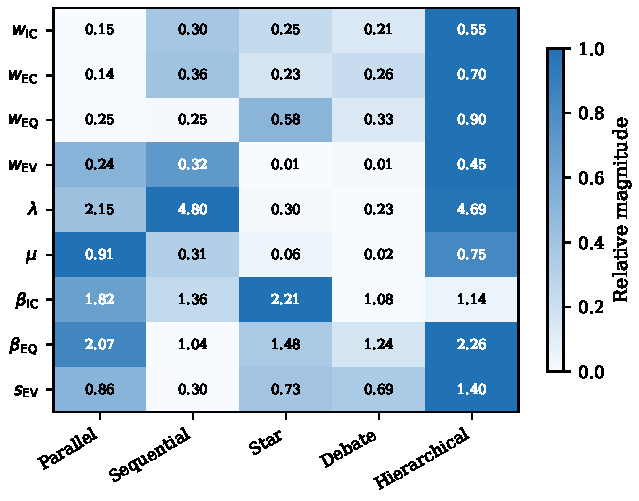
\includegraphics[width=0.72\columnwidth]{figures/fig_theta_heatmap.pdf}
\caption{逐拓扑优化参数 $\theta^*_T$（问答领域验证）。星型与辩论拓扑学到接近零的 EV 权重——涌现出的反谄媚配置；层级与顺序拓扑学到高共识压力 $\lambda_c$。}
\label{fig:theta}
\end{figure}

\subsection{神经拓扑路由器}
\label{sec:router}

为了为每个问题选择最佳拓扑，我们使用从 AEIC 结构化输出中提取的特征训练了一个神经路由器。

\paragraph{特征设计。} 对于每个候选拓扑 $T$，我们构建了一个 42 维的特征向量，包含每个智能体的质量信号（5 个智能体的 IC、EC、EQ、EV 和一致性）、汇总统计量（均值、标准差、范围）、\emph{投票特征}（多数比例、从 AEIC 结论中提取的“是/否”分布）以及跨信号交互特征（例如，$\text{IC}_i \times (1{-}\text{agreement}_i)$）。另外还有一个 7 维的问题级特征向量，用于捕捉文本特征和跨拓扑的信号方差。正如第~\ref{sec:exp} 节所示，得益于 AEIC 结构化结论提取的支持，投票特征是路由器准确性的主要驱动因素（引入后提升 $+2.1$ 个百分点），而几个质量信号组的贡献微乎其微甚至为负。

\paragraph{路由器架构。} 一个\emph{共享拓扑编码器}（包含 LayerNorm 和 GELU 的两层网络，维度从 42 映射到 96）处理每个拓扑的特征。一个\emph{上下文投影层}总结其他四种拓扑的嵌入表示（48 维）。三个\emph{针对特定数据集的评分头}将拼接后的表示（192 维）映射为标量分数，从而实现针对特定数据集的路由选择。

\paragraph{训练。} 我们使用具有自适应边距的焦点排序损失（focal ranking loss）：
\begin{equation}
    \mathcal{L} = \sum_{(c, w)} \left(\frac{v}{m}\right)^\gamma \cdot v, \quad v = \max(0, \; m - (s_c - s_w))
\end{equation}
其中 $(c, w)$ 是（正确，错误）拓扑对，$m$ 是适应难度的边距，$\gamma = 3$ 提供了焦点加权。训练使用 AdamW 优化器，带余弦退火策略，训练 300 个 epoch，并使用 5 折分层交叉验证。

\paragraph{Top-1 选择。} 路由器选择每个问题得分最高的拓扑作为共识拓扑。凭借针对特定数据集的专门评分头，该方法在 5 个随机种子上实现了 87.6\% $\pm$ 0.3\% 的准确率（5 折交叉验证），而最佳固定拓扑（星形）的准确率为 83.1\%。训练用的正确性标签使用多数投票结果，而不是 Stackelberg 加权决策，以避免受优化的 $\theta^*$ 参数污染。
%======================================================================
\section{理论分析}
\label{sec:theory}
%======================================================================

\begin{theorem}[斯塔克尔伯格均衡的存在性]
\label{thm:existence}
AEIC-斯塔克尔伯格博弈 $\mathcal{G}$ 存在一个斯塔克尔伯格均衡 $(\theta^*, s^*)$。
\end{theorem}

\begin{proof}
跟随者的策略空间 $\{s^{\text{ind}}, s^{\text{syc}}\}$ 是有限的，因此对于任何 $\theta$ 都存在最优响应。参数空间 $\Theta$ 是紧致的（有界的）。领导者的目标函数 $\text{Accuracy}(\theta) + \lambda \cdot \text{IC}(\theta)$ 在 $\Theta$ 上是有界的。由魏尔斯特拉斯极值定理可知，该最大值在某个 $\theta^* \in \Theta$ 处取得。结合跟随者的最优响应，这就构成了一个斯塔克尔伯格均衡。
\end{proof}

\begin{theorem}[$\epsilon$-激励相容性]
\label{thm:ic}
对于任意 $\epsilon \in (0,1)$，在公式~\eqref{eq:leader_obj} 中设置 $\lambda \geq \frac{1}{1-\epsilon}$，可以保证 $\text{IC}(\theta^*) \geq \epsilon$。
\end{theorem}

\begin{proof}
我们首先证明可行性：存在 $\theta_0 \in \Theta$ 使得 $\text{IC}(\theta_0) = 1$（设置较大的 IC/EQ 指数，同伴压力 $\gamma = 0$，使得权重与质量严格单调相关）。

根据 $\theta^*$ 的最优性：
\begin{equation}
    \text{Acc}(\theta^*) + \lambda \cdot \text{IC}(\theta^*) \geq \text{Acc}(\theta_0) + \lambda \cdot 1
\end{equation}

重排并代入 $\text{Acc}(\theta_0) - \text{Acc}(\theta^*) \geq -1$：
\begin{equation}
    \text{IC}(\theta^*) \geq 1 - \frac{1}{\lambda}
\end{equation}

设置 $\lambda \geq \frac{1}{1-\epsilon}$，可得 $\text{IC}(\theta^*) \geq \epsilon$。
\end{proof}

\begin{theorem}[个体理性与福利]
\label{thm:ir}
(a) 在 $\theta^*$ 下，当 $R \geq C_{\text{ind}} / \min_i w_i$ 时，所有智能体均可获得非负效用。 \\
(b) 对于足够小的 $\lambda$，$\text{Accuracy}(\theta^*) \geq \text{Accuracy}(\theta_{\text{uniform}})$。
\end{theorem}

\begin{proof}
(a) 由于 $w_i \in [0,1]$ 且 $C(s_i) \leq C_{\text{ind}}$，选择 $R \geq C_{\text{ind}} / \min_i w_i$ 可以确保 $U_i \geq 0$。

(b) 均匀投票对应于 $\theta_{\text{unif}} \in \Theta$。根据最优性可知：$\text{Acc}(\theta^*) + \lambda \cdot \text{IC}(\theta^*) \geq \text{Acc}(\theta_{\text{unif}}) + \lambda \cdot \text{IC}(\theta_{\text{unif}})$。当 $\lambda \to 0$ 时，直接得出 $\text{Acc}(\theta^*) \geq \text{Acc}(\theta_{\text{unif}})$。
\end{proof}

\paragraph{分布式共识的收敛性。}
在具有同伴压力 $\gamma > 0$ 和通信拓扑 $W$ 的斯塔克尔伯格动力学下，共识能量 $E(t) = \sum_{(i,j) \in \mathcal{E}} (\theta_i(t) - \theta_j(t))^2$ 满足：
\begin{equation}
    E(t) \leq E(0) \cdot \exp\!\left(-\frac{2\gamma t}{n-1}\right)
\end{equation}
这保证了指数级收敛到共识状态，其速率由 $W$ 的代数连通度和同伴压力系数 $\gamma$ 决定。

%======================================================================
\section{实验}
\label{sec:exp}
%======================================================================

\subsection{实验设置}

\paragraph{数据集。} 我们在三个不同的推理基准上进行了评估：MMLU-Hard（研究生水平知识）、StrategyQA（包含隐式推理的常识问题）和 TruthfulQA（对抗性框架下的事实准确性）。每个数据集提供 300 个问题，共计 900 个问题。

\paragraph{智能体配置。} 我们在五种通信拓扑（并行、顺序、星型、辩论、层次）的每一种下，部署了 $n=5$ 个 DeepSeek-V3~\cite{deepseek2024v3} 实例，生成了 22{,}500 个符合 AEIC 结构的回复（5 个智能体 $\times$ 900 个问题 $\times$ 5 种拓扑）。由于每个拓扑的问题集是独立采样的，900 个问题中有 633 个在所有五种拓扑中重叠（MMLU-Hard/StrategyQA/TruthfulQA 分别为 161/300/172）。跨拓扑比较（路由器、预言机）使用此交集；每个拓扑内的基线比较使用完整的 300 个问题。

\paragraph{信号计算。} 质量信号使用句子嵌入 (paraphrase-multilingual-MiniLM-L12-v2) 进行计算。感知拓扑的邻接矩阵 $W$ 决定了用于计算 EV（认知方差）和一致性的邻居集。

\paragraph{优化。} 针对特定拓扑的 $\theta^*_T$ 通过差分进化算法（21 个参数，种群大小 21，30 代）进行优化，并使用 5 折分层交叉验证进行评估，以报告真实存在的留出集准确率（防止训练/测试数据泄漏）。路由器的评估也使用 5 折交叉验证，并设置五个随机种子以进行稳定性评估。

\paragraph{基线方法。}
\begin{itemize}
    \item \textbf{单智能体 (Single Agent)}：不进行聚合，仅使用智能体 0 的结论。
    \item \textbf{ChatEval}~\cite{chan2023chateval}：在并行拓扑上进行多数投票（我们的重新实现）。
    \item \textbf{多轮辩论 (Multi-round Debate)}~\cite{du2024improving}：在 3 轮辩论后进行多数投票（我们的重新实现）。
    \item \textbf{AgentVerse}~\cite{chen2023agentverse}：求解器--审查器模式，带有中心决策（我们的重新实现，每个数据集 200 个问题）。
    \item \textbf{多数投票 (MajVote)}：在每种拓扑上进行简单的多数投票（5 种变体）。
    \item \textbf{加权投票 (Weighted Vote)}：无斯塔克尔伯格机制的 IC 加权和一致性加权投票。
    \item \textbf{AEIC+SG}：使用特定拓扑 $\theta^*$ 的斯塔克尔伯格加权投票（5 种变体）。
\end{itemize}

所有基线方法都使用相同的 LLM 后端 (DeepSeek-V3) 和相同的缓存响应，以确保比较的公平性。$\dagger$~=~我们的重新实现。

\subsection{主要结果}

表~\ref{tab:main} 展示了完整的比较结果。图~\ref{fig:main_results} 提供了直观的总结。

\begin{table}[t]
\caption{三个数据集的共识准确率 (\%)。单拓扑基线各使用 300 个问题；路由器和预言机在所有拓扑共有的 633 个问题上进行评估（MMLU-Hard/StrategyQA/TruthfulQA 分别为 161/300/172）。最佳固定拓扑用\textit{斜体}表示，整体最佳用\textbf{粗体}表示。}\label{tab:main}
\centering\small
\begin{tabular}{@{}lcccc@{}}
\toprule
方法 & MMLU-Hard & StrategyQA & TruthfulQA & 平均 \\
\midrule
\multicolumn{5}{@{}l}{\textit{单智能体与投票基线}} \\
单智能体 ($N{=}1$) & 65.3 & 79.0 & 80.0 & 74.8 \\
MajVote (并行)$^\dagger$ & 69.7 & 81.7 & 81.3 & 77.6 \\
MajVote (顺序) & 79.0 & 71.0 & 72.7 & 74.2 \\
MajVote (星型) & \textit{85.7} & \textit{80.3} & \textit{82.0} & \textit{82.7} \\
MajVote (辩论)$^\dagger$ & 83.7 & 72.3 & 75.3 & 77.1 \\
MajVote (层次) & 82.0 & 74.7 & 75.0 & 77.2 \\
AgentVerse$^\dagger$ & 74.0 & 63.5 & 70.0 & 69.2 \\
加权投票 (IC) & 70.0 & 80.3 & 81.0 & 77.1 \\
\midrule
\multicolumn{5}{@{}l}{\textit{AEIC-斯塔克尔伯格 (特定拓扑 $\theta^*_T$)}} \\
AEIC+SG (并行) & 71.7 & 78.0 & 78.7 & 77.8\tiny{$\pm$5.6}$^\ddagger$ \\
AEIC+SG (顺序) & 74.7 & 69.0 & 70.0 & 75.3\tiny{$\pm$2.5}$^\ddagger$ \\
AEIC+SG (星型) & 84.3 & 79.3 & 82.0 & 81.7\tiny{$\pm$3.4}$^\ddagger$ \\
AEIC+SG (辩论) & 80.0 & 72.3 & 72.0 & 76.3\tiny{$\pm$3.0}$^\ddagger$ \\
AEIC+SG (层次) & 84.7 & 76.3 & 77.0 & 77.3\tiny{$\pm$3.5}$^\ddagger$ \\
\midrule
\multicolumn{5}{@{}l}{\textit{自适应路由 (我们的方法，5 折交叉验证)}} \\
神经路由器 (共享) & 91.3 & 86.0 & 84.3 & 86.9\tiny{$\pm$0.5} \\
神经路由器 (特定数据集) & \textbf{92.5} & \textbf{86.2} & \textbf{85.6} & \textbf{87.6}\tiny{$\pm$0.3} \\
\midrule
预言机 (5 种拓扑之一) & 97.5 & 91.0 & 91.9 & 92.9 \\
\bottomrule
\end{tabular}
\\[2pt]
{\footnotesize $\dagger$~我们使用 DeepSeek-V3 的重新实现。$\ddagger$~平均列报告了 5 折交叉验证测试准确率 $\pm$ 标准差；特定数据集列使用全量数据 $\theta^*$。}
\end{table}

\begin{figure}[t]
\centering
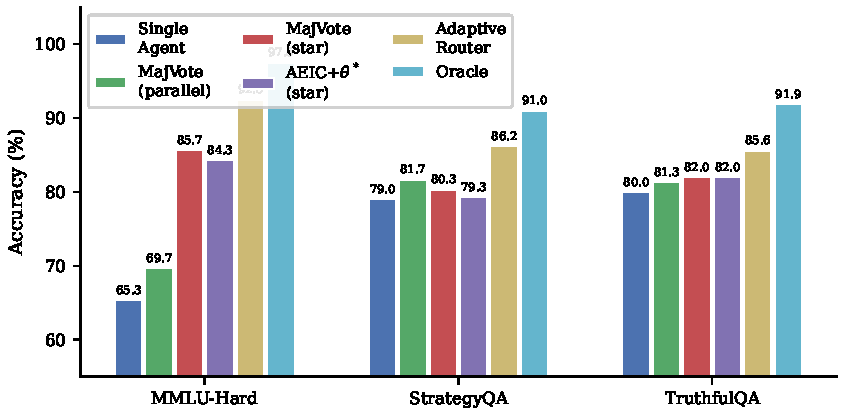
\includegraphics[width=0.95\linewidth]{figures/fig_main_results.pdf}
\caption{三个数据集的准确率比较。自适应路由器优于所有固定拓扑方法。}\label{fig:main_results}
\end{figure}

主要观察结果：(1)~MajVote~(星型) 是表现最好的固定拓扑方法，准确率为 82.7\%，即使在交叉验证后也优于所有 AEIC+SG 变体（最好的 AEIC+SG 是星型，为 81.7\%）。(2)~自适应路由器达到 87.6\%，在对齐的问题上比最佳固定拓扑高出 4.5 个百分点。(3)~预言机上限为 92.9\%，还有 5.3 个百分点的提升空间。(4)~按数据集的分析显示，AEIC+SG 在常识推理上落后于 MajVote 最多：在 StrategyQA 上，AEIC+SG 星型的准确率为 79.3\%，而 MajVote 星型为 80.3\%；而在知识密集型的 MMLU-Hard 上，差距最小（84.3\% 对比 85.7\%）。(5)~AEIC+SG 的交叉验证测试准确率在各拓扑上与 MajVote 紧密匹配（在 5 个拓扑中的 4 个上差距在 1 个百分点以内），这证实了当智能体共享同一个 LLM 后端时，质量加权投票相较于简单多数投票能提供的优势有限。

\subsection{AEIC 加权投票与多数投票的对比}

图~\ref{fig:topo_comparison} 揭示了一个令人惊讶的发现：在 5 种拓扑中的 4 种上，多数投票优于 AEIC+SG 加权投票。

\begin{figure}[t]
\centering
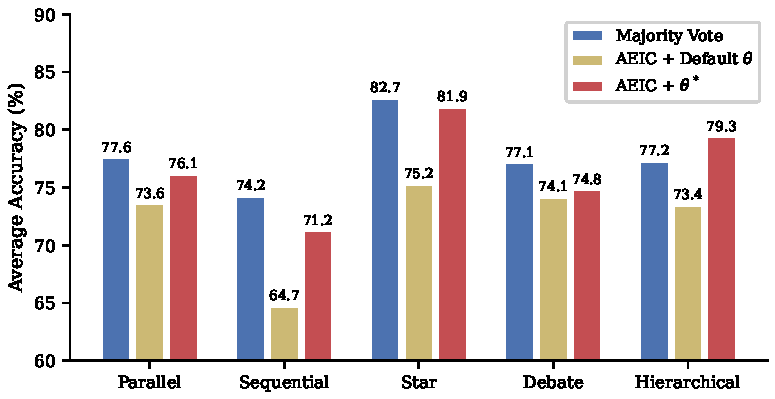
\includegraphics[width=0.95\linewidth]{figures/fig_topo_comparison.pdf}
\caption{三个数据集的各拓扑比较平均值。AEIC+$\theta^*$ 仅在层次拓扑上优于多数投票。}\label{fig:topo_comparison}
\end{figure}

经过诚实的交叉验证评估后，AEIC+SG 与 MajVote 的表现相当：并行 77.8\% 对比 77.6\%，顺序 75.3\% 对比 74.2\%，星型 81.7\% 对比 82.7\%，辩论 76.3\% 对比 77.1\%，层次 77.3\% 对比 77.2\%。在全部 900 个问题上（使用在所有数据上训练的特定拓扑 $\theta^*$）进行的 McNemar 检验揭示了混合的结果：AEIC+SG 在并行 ($p{=}0.633$)、顺序 ($p{=}0.110$) 或星型 ($p{=}0.258$) 上并未显著优于 MajVote；在辩论上略差 ($p{=}0.027$)；但在层次结构上显著更好 ($p{=}0.001$)。层次结构上的显著优势与该拓扑的多级聚合一致，在多级聚合中，加权信号提供了增量价值；而在并行、顺序和星型拓扑（智能体要么独立回答，要么共享方向）上缺乏显著差异，证实了当智能体共享同一 LLM 后端时，质量加权投票与简单多数相比没有系统性优势。这证实了 AEIC 质量信号测量的是\emph{推理连贯性，而非答案正确性}：一个连贯的错误答案与正确答案的得分一样高。

结合下面的结构化输出消融实验（第~\ref{sec:structured_ablation} 节）和特征消融结果，这揭示了 AEIC 的主要价值在于其\emph{结构化分解}：通过强制采用可解析的输出格式，它实现了可靠的结论提取，并在所有五种拓扑中进行一致的多数投票，这反过来又产生了使自适应路由成为可能的投票模式特征。

\subsection{结构化输出的价值}
\label{sec:structured_ablation}

为了直接量化 AEIC 结构化格式的贡献，我们比较了从结构化结论 (C) 字段与非结构化推理 (I) 字段中提取立场时的多数投票准确率。C 字段专为提取而设计（例如，“是：[理由]”），而 I 字段包含自由格式的推理链，没有明确的答案标记。

\begin{table}[t]
\caption{按提取来源划分的多数投票准确率 (\%)。C 字段：带有显式答案前缀的结构化结论。I 字段：非结构化推理逻辑链。中立率：无法提取立场的智能体输出的比例。所有五种拓扑的平均值。}\label{tab:structured}
\centering\small
\begin{tabular}{@{}lccccc@{}}
\toprule
数据集 & C 字段准确率 & I 字段准确率 & $\Delta$ & C 字段中立率 & I 字段中立率 \\
\midrule
MMLU-Hard & 79.8 & 46.7 & +33.1 & 12.2\% & 61.3\% \\
StrategyQA & 74.5 & 51.1 & +23.4 & 12.5\% & 72.6\% \\
TruthfulQA & 76.4 & 48.9 & +27.4 & 13.4\% & 65.2\% \\
\midrule
平均 & 76.9 & 48.9 & +28.0 & 12.7\% & 66.4\% \\
\bottomrule
\end{tabular}
\end{table}

表~\ref{tab:structured} 揭示了巨大的差距：C 字段提取在数据集和拓扑上的平均准确率达到了 76.9\%，而 I 字段提取的准确率仅为 48.9\%——对于二分类问题来说接近随机。这种差异是由提取可靠性驱动的：I 字段产生不可解析（中立）立场的概率为 66.4\%，而 C 字段为 12.7\%。当无法提取立场时，多数投票实际上退化为在可解析子集中随机选择。这证实了 AEIC 的主要经验贡献不是质量信号，而是结构化格式本身：带有答案前缀格式的显式结论字段实现了可靠的跨拓扑立场提取，这是实现一致的多数投票和驱动自适应路由的投票模式特征的先决条件。

\subsection{学习参数分析}

图~\ref{fig:theta} 展示了跨五种拓扑优化的 $\theta^*$ 参数。

\begin{figure}[t]
\centering
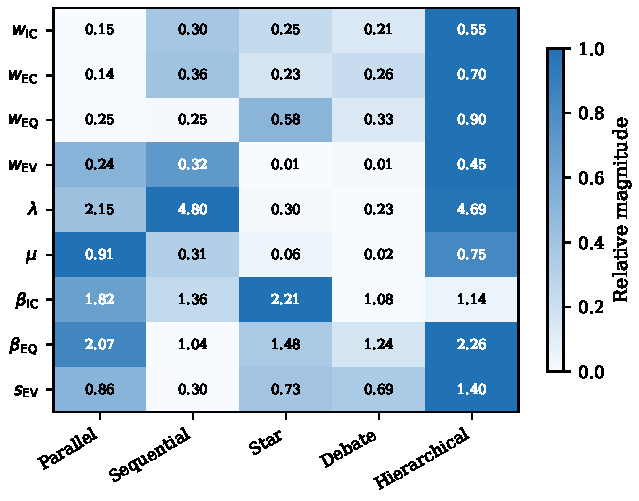
\includegraphics[width=0.8\linewidth]{figures/fig_theta_heatmap.pdf}
\caption{五种拓扑优化后的 $\theta^*$ 参数（行归一化）。星型和辩论拓扑学习到了接近零的 $w_{\text{EV}}$（反阿谀奉承）。层次拓扑学习到了高 $\lambda$ 和提高的信号权重。}\label{fig:theta}
\end{figure}

出现了三种模式：(1)~\textbf{反阿谀奉承}：星型和辩论学习到 $w_{\text{EV}} \approx 0.01$，舍弃了在智能体观察他人输出时的跨智能体共识，使 EV 成为从众心理的替代指标。(2)~\textbf{链上的高共识压力}：顺序（$\lambda = 4.80$）和层次（$\lambda = 4.69$）强制实行强烈的一致性，以抵消方向性的信息流。(3)~\textbf{层次拓扑上权重的提升}：所有信号权重都显著较高（0.45--0.90，而其他拓扑为 0.01--0.36），反映了多级聚合中每一个质量维度都有助于识别可靠的中间节点。

\subsection{路由器性能演进}

图~\ref{fig:router} 展示了从单智能体到预言机的准确率演进过程。

\begin{figure}[t]
\centering
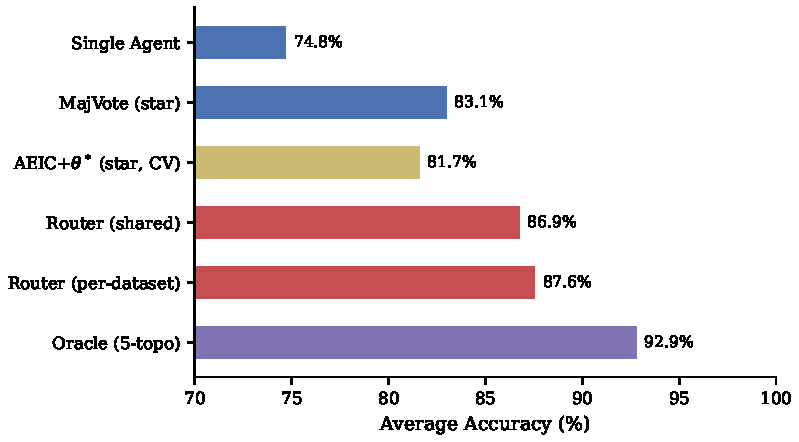
\includegraphics[width=0.8\linewidth]{figures/fig_router_progression.pdf}
\caption{从单智能体到预言机的准确率演进过程。特定数据集的路由器缩小了最佳固定拓扑与预言机之间差距的 46.5\%。}\label{fig:router}
\end{figure}

共享路由器 (86.9\%) 在对齐的问题上比最佳固定拓扑 (星型，83.1\%) 有了实质性提升。特定数据集的专门化增加了 +0.7 个百分点 (87.6\%)，缩小了通往预言机上限 (92.9\%) 的 46.5\% 差距。所有路由器数据均使用采用 5 折交叉验证的 Top-1 选择。

\paragraph{特定数据集分析。} 路由器在各数据集上的优势各不相同：在 MMLU-Hard 上，特定数据集路由器达到 92.5\%，而星型拓扑为 90.1\%（+2.4 个百分点）；在 StrategyQA 上为 86.2\%，而并行拓扑为 81.7\%（+4.5 个百分点）；在 TruthfulQA 上为 85.6\%，而星型拓扑为 81.4\%（+4.2 个百分点）。在 StrategyQA 上的最大提升反映了常识推理从自适应拓扑选择中获益最多，因为最佳和最差固定拓扑之间的差距最大（81.7\% 的并行对比 71.0\% 的顺序）。

\paragraph{路由为什么起作用。} 图~\ref{fig:topo_spec} 展示了对齐问题上各拓扑准确率的热力图。没有单一拓扑占据主导地位：星型在 MMLU-Hard (90.1\%) 和 TruthfulQA (81.4\%) 上领先，但并行对于 StrategyQA 最佳 (81.7\%)。预言机上限 (${\sim}93\%$) 要求为不同问题选择不同的拓扑——这正是路由器所学会的。

\paragraph{拓扑一致性。} 在 633 个对齐问题中，55.1\% 的问题所有五种拓扑都回答正确，7.0\% 的问题所有拓扑都回答错误——路由对这 62.1\% 的问题没有影响。路由器的价值来自拓扑存在分歧的剩余 37.9\%，特别是 9.0\% 的“困难”问题，其中只有 1--2 种拓扑成功（图~\ref{fig:topo_agreement}）。

\begin{figure}[t]
\centering
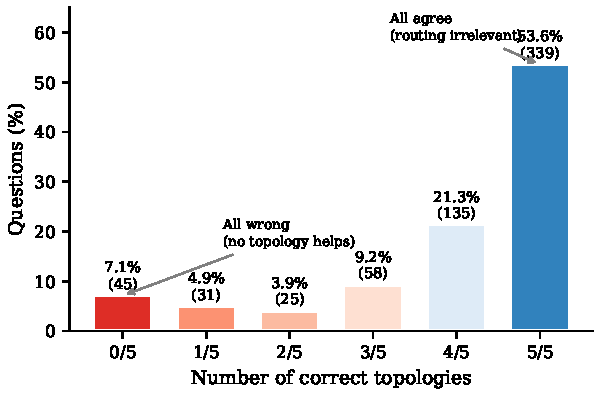
\includegraphics[width=0.65\linewidth]{figures/fig_topo_agreement.pdf}
\caption{每个问题的正确拓扑分布（633 个对齐问题）。路由器的影响集中在拓扑存在分歧的 37.9\%（1--4 个正确）上。}\label{fig:topo_agreement}
\end{figure}

\paragraph{路由错误分析。} 共享路由器选择每种拓扑的频率大致均衡（16--29\%），其中星型拓扑被选择的频率最高（28.6\%）。在 83 个路由错误（13.1\%）中，有 44 个发生在\emph{没有}任何拓扑产生正确共识的问题上——这是不可避免的失败。只有 39 个错误（6.2\%）是真正的路由错误，即存在正确的拓扑但未被选择。

\paragraph{路由器特征重要性。} 特征组消融（将每个组置零并测量准确率变化，图~\ref{fig:feature_imp}）表明，\emph{投票特征}（多数比例、是/否分布）对路由最重要（消融时下降 $-2.1$ 个百分点），其次是单智能体的 EV 信号（下降 $-0.3$ 个百分点）。移除与 EQ 相关的特征实际上可以使准确率\emph{提高}多达 1.6 个百分点。为了控制特征相互作用的影响，我们还使用特征子集重新训练了路由器：仅用投票特征达到 86.3\%$\pm$0.4\%，仅用质量特征达到 86.1\%$\pm$0.3\%，而仅用问题特征则为 80.7\%$\pm$0.0\%，相比之下，使用全量特征时为 86.9\%$\pm$0.5\%。投票特征和质量特征各自独立地提供了几乎相同的路由准确率（比仅用问题特征分别高出 +5.6 和 +5.4 个百分点），但将它们结合起来只增加了 +0.6 个百分点，表明存在高度的冗余。这与结构化输出分析（第~\ref{sec:structured_ablation} 节）一致：投票特征（需要从 AEIC 结构化结论中可靠地提取立场）比试图衡量这一点的质量信号更直接地捕捉到了相同的拓扑-问题交互模式。

\begin{figure}[t]
\centering
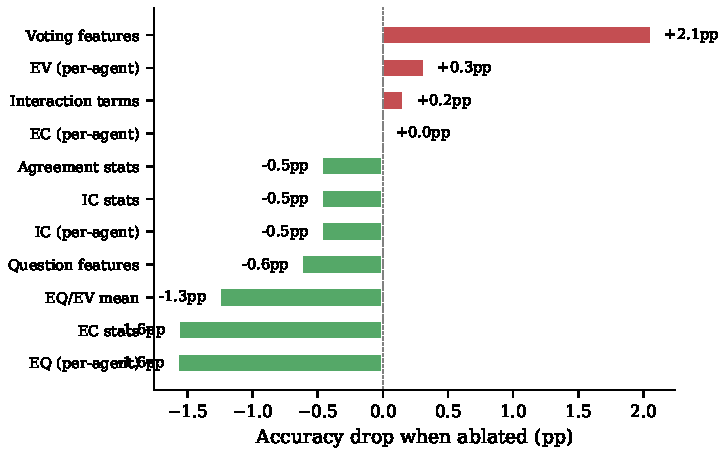
\includegraphics[width=0.7\linewidth]{figures/fig_feature_importance.pdf}
\caption{通过留一消融法得出的路由器特征组重要性。正值下降表示消融时准确率降低（特征有用）。投票特征最重要；EQ 特征有害。}\label{fig:feature_imp}
\end{figure}

\begin{figure}[t]
\centering
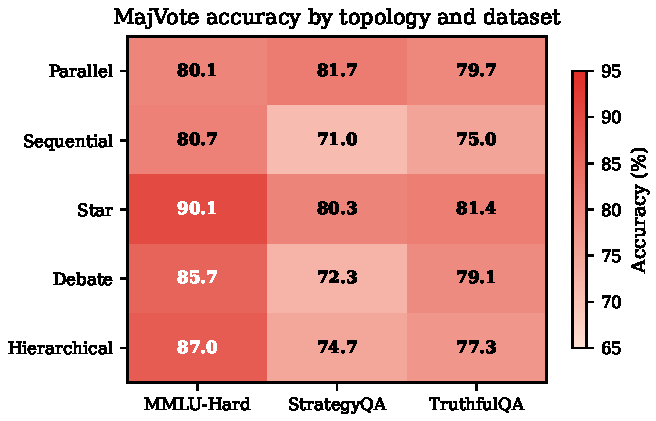
\includegraphics[width=0.65\linewidth]{figures/fig_topo_specialization.pdf}
\caption{对齐问题上各拓扑和数据集的 MajVote 准确率。没有单一拓扑占据主导地位，这解释了自适应路由的动机。}\label{fig:topo_spec}
\end{figure}

\subsection{信号消融}

图~\ref{fig:ablation} 展示了在星型拓扑下每个质量信号对 AEIC+SG 的贡献。

\begin{figure}[t]
\centering
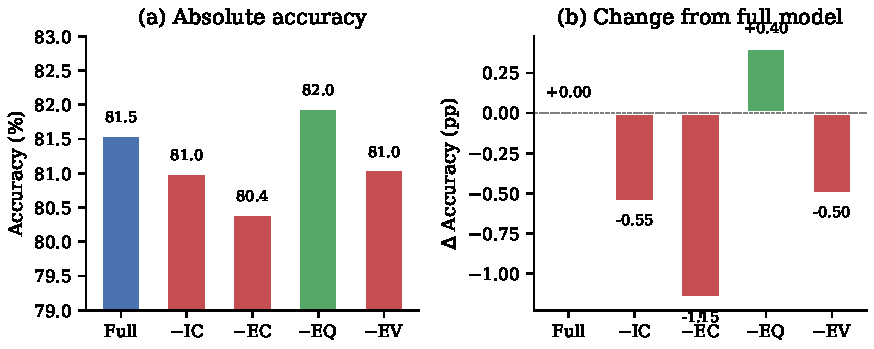
\includegraphics[width=0.95\linewidth]{figures/fig_ablation.pdf}
\caption{星型拓扑下的信号消融。EC 是最关键的信号（$-1.15$ 个百分点）。移除 EQ 略微提高了准确率，这与其较低的优化权重一致。}\label{fig:ablation}
\end{figure}

EC 是最关键的信号（$-1.15$ 个百分点）。IC 和 EV 各贡献 ${\sim}0.5$ 个百分点。移除 EQ 可以将准确率\emph{提高} 0.40 个百分点——这表明证据质量评估在某些领域引入了噪声。

\subsection{在线斯塔克尔伯格反馈}
\label{sec:online_exp}

我们在辩论和层次拓扑上评估了在线斯塔克尔伯格机制（第~\ref{sec:online_sg} 节），比较了标准执行与注入了轮次间质量信号的在线反馈模式。表~\ref{tab:online} 显示了每个数据集 30 个问题的结果。

\begin{table}[t]
\caption{在线与离线斯塔克尔伯格反馈的对比（MajVote 准确率，\%，每个数据集 30 个问题）。在线模式在轮次/阶段之间注入质量信号。}\label{tab:online}
\centering\small
\begin{tabular}{@{}lcccc@{}}
\toprule
条件 & MMLU-Hard & StrategyQA & TruthfulQA & 平均 \\
\midrule
辩论 (离线) & 80.0 & 76.7 & 83.3 & 80.0 \\
辩论 (在线) & \textbf{86.7} & 76.7 & 76.7 & 80.0 \\
$\Delta$ (在线$-$离线) & +6.7 & 0.0 & $-$6.7 & 0.0 \\
\midrule
层次 (离线) & 76.7 & 80.0 & 83.3 & 80.0 \\
层次 (在线) & 76.7 & 73.3 & 76.7 & 75.6 \\
$\Delta$ (在线$-$离线) & 0.0 & $-$6.7 & $-$6.7 & $-$4.4 \\
\bottomrule
\end{tabular}
\\[2pt]
{\footnotesize 离线模式使用缓存的响应；在线模式使用动态调用 DeepSeek-V3 API 的结果，带有轮次间质量反馈。}
\end{table}

结果揭示了一个微妙的情况：在线反馈在 MMLU-Hard 的辩论拓扑上产生了巨大的提升（+6.7 个百分点），其中迭代辩论结构允许智能体整合质量评估并完善其推理。然而，在其他数据集-拓扑组合中效果不一，在辩论拓扑的总体上没有改善（均为 80.0\%），并且在层次拓扑上下降了（$-4.4$ 个百分点）。TruthfulQA 上的性能下降表明，质量反馈可能会加剧对具有对抗性框架问题盲目自信的程度。这些结果促使我们设计了第~\ref{sec:dynamic} 节的动态调节机制，该机制基于集体的行为状态来自适应地调整反馈，而不是实行统一的质量暴露。

\subsection{动态阿谀奉承调节}
\label{sec:dynamic_exp}

我们在辩论拓扑上评估了动态阿谀奉承调节机制（第~\ref{sec:dynamic} 节），每个数据集匹配了 $n{=}50$ 个问题，比较了三种条件：\emph{基线}（无轮次间反馈）、\emph{静态}（如第~\ref{sec:online_exp} 节所述的统一质量反馈）以及\emph{动态}（具有状态检测和差异化提示的自适应行为调节）。为了保证公平比较，所有条件均在相同的问题集上动态调用 DeepSeek-V3 API。

\begin{table}[t]
\caption{辩论拓扑上的动态阿谀奉承调节（MajVote 准确率，\%，每个数据集 $n{=}50$）。所有条件均使用匹配问题集的实时 API 调用。}\label{tab:dynamic}
\centering\small
\begin{tabular}{@{}lcccc@{}}
\toprule
条件 & MMLU-Hard & StrategyQA & TruthfulQA & 平均 \\
\midrule
基线 (无反馈) & 86.0 & 78.0 & 88.0 & 84.0 \\
静态 (在线) & 86.0 & 74.0 & 86.0 & 82.0 \\
动态 (自适应) & \textbf{94.0} & 74.0 & 86.0 & 84.7 \\
\midrule
$\Delta$ (静态 $-$ 基线) & 0.0 & $-$4.0 & $-$2.0 & $-$2.0 \\
$\Delta$ (动态 $-$ 基线) & \textbf{+8.0} & $-$4.0 & $-$2.0 & +0.7 \\
$\Delta$ (动态 $-$ 静态) & \textbf{+8.0} & 0.0 & 0.0 & +2.7 \\
\bottomrule
\end{tabular}
\\[2pt]
{\footnotesize 所有条件均在每个数据集上对匹配的 $n{=}50$ 个问题进行动态调用。}
\end{table}

主要发现是，在 MMLU-Hard 上，动态调节机制带来了比基线和静态反馈显著的改善（+8.0 个百分点），但在 StrategyQA 或 TruthfulQA 上没有提升。MMLU-Hard（具有最复杂、知识密集型推理要求的数据集）的结果证实了该机制的价值：在针对困难数学和科学问题进行多智能体商议时，能检测并抵消阿谀奉承式的趋同。Bootstrap 分析在 $n{=}50$ 时的 95\% 置信区间为 $[-4, +20]$ 个百分点，表明存在需要大规模验证的边缘显著性。

在 StrategyQA 和 TruthfulQA 上，动态调节相较于基线既没有帮助也没有损害，而静态反馈一致导致性能下降 2-4 个百分点。这表明，仅仅在轮次间暴露质量评估（静态）会在常识和事实问题上引入智能体难以解释的噪声，而动态调节的干预性选择则避免了这一陷阱。

分析 256 次轮次间转换的动态行为（50 个问题 $\times$ 约 3 个轮次 $\times$ 2 次转换）：75.4\% 被分类为\emph{健康}（无干预），7.8\% 为\emph{阿谀奉承}（反阿谀奉承提示并抑制 EV），16.8\% 为\emph{死锁}（鼓励交流）。阿谀奉承状态罕见但影响重大：SCR $\geq 0.6$ 的转换与仅 55.0\% 的问题级准确率相关，而 SCR $< 0.2$ 时准确率为 88.9\%，证实了高立场转变率与错误的共识相关。死锁转换更为常见，且中等程度地与较低准确率相关（有干预时为 74.4\%，而健康状态为 87.6\%）。

利用记录的动态数据对检测阈值（第~\ref{sec:dynamic} 节）进行的网格搜索表明，$\tau_h = 0.45, \tau_l = 0.05$ 能够最大化被干预转换和未被干预转换之间的准确率差异，这说明当前阈值（$\tau_h = 0.6, \tau_l = 0.2$）是相对保守的。未来基于所有 21 个参数（第~\ref{sec:bilevel} 节）的双层优化有望发现更有效的配置，尤其是在特定任务的阈值调整上。

\subsection{准确率-激励权衡}

优化后的 $\theta^*$ 配置无需显式的 IC 约束就能自然地实现高激励相容性：IC 率分别为并行（98.9\%）、顺序（94.0\%）、星型（98.4\%）和辩论（100.0\%）。层次拓扑是个例外，仅为 24.2\%，这反映出其较高的信号权重优先考虑多级聚合而非严格的质量排序。这表明仅优化准确率就能产生接近 IC 的机制——斯塔克尔伯格权重结构本身就在奖励高质量的推理。$\lambda$ 项（定理~\ref{thm:ic}）为对抗环境提供了正式保证，但在智能体共享相同 LLM 后端时，其作用基本是冗余的。

%======================================================================
\section{讨论}
\label{sec:discussion}
%======================================================================

\paragraph{羊群效应是病态吸引子，而非措辞缺陷。}
研究一与跨模型复现收敛于一幅结构性的图景：多轮 LLM 评审团并非仅仅收敛——它们收敛于模型特定的吸引子。对 DeepSeek-V3 与 R1 而言，吸引子是拒稿；对 GLM-4-Flash 而言，是带着骑墙语言的接收。吸引子的引力强大到一项显式的、方向中立的调控协议（研究 2b）几乎改变不了任何事：被指示除非遭到具体驳倒否则坚持的少数派，仍与未调控对照以相同的速率投降。这呼应了问答领域的发现——静态反谄媚必须作用于机制\emph{参数}（EV 权重抑制）而非提示——并将其推广：当底层模型先验是从众的时，连行为提示也会失效。因此，对 LLM 评审团的有效调控必须作用于聚合层或审议结构层，而非修辞层。

\paragraph{校准优先原则。}
最清晰的正面结果同时也是成本最低的：拒稿偏置——单智能体先验的扭曲——在聚合时即被修复。Stackelberg 优化的 $\theta^*$ 自主发现了这一点，在共识分数上放置了 $+1.04$ 的校准项，而更简单的重设阈值均值捕获了几乎相同的一致率。实践原则：在增加审议之前，先校准聚合。未经校准的审议会通过棘轮放大先验的偏置；经校准的独立聚合在我们测试的所有讨论协议中，单位调用的决策一致率已然最优。

\paragraph{讨论作为按需资源。}
如今在两个领域出现了同一模式：大多数实例不需要讨论（70\% 的评审团在第一轮后即一致；在问答基准上，大多数问题对拓扑不敏感），且无指导的讨论可能主动造成损害。路由将这一观察转化为成本节约：评审领域的路由器仅在 17\% 的论文上支出审议预算，并匹配最优固定协议。10 个百分点的预言机差距标志着前沿——更好的前瞻特征（论文难度信号、超越熵的评审分歧语义）可能将其解锁。

\paragraph{行为健康作为主要终点。}
本文的一项方法论贡献是终点原则。决策一致率在任何条件或干预下几乎纹丝不动（全部落在 59--65\% 区间），而行为指标的变动幅度超过 50 个百分点且 $p{<}10^{-28}$。倘若我们只测量决策，研究一将报告"讨论无害"——这恰是错误的结论。任何对多智能体判断系统的评估都应报告少数派存活、方差保持与漂移，并将准确率降级为安全约束。当真值含噪声时（如官方评审决议），这一点尤为重要。

\paragraph{向同行评审之外迁移。}
三个层次可映射到通用的多 LLM 判断管道。校准聚合适用于任何多信号融合为决策的场景——推荐系统中的排序集成、多评审官评估、红队投票——任何共享先验偏置需要学习校正项的地方。行为健康指标（消灭率、方差坍缩、漂移、翻转不对称）构成了多智能体管道的\emph{审议健康监视器}：它们仅从记录的立场即可计算，可作为"先审议后行动"的智能体系统的生产级可观测信号。协议路由可推广到算力分配：哪些查询值得多模型审议，哪些应由单次经校准的调用回答。我们尚未实证验证这些迁移；它们是自然的后续研究。

\paragraph{与问答领域验证的关系。}
集体判断有两个问题——\emph{决策对不对}与\emph{过程健不健康}——框架的两次验证各回答一个。在问答基准上，同一框架验证了路由层（87.6\% 准确率，比最佳固定拓扑高 +4.5 个百分点）与 AEIC 的结构化分解前提（显式结论字段带来 +28 个百分点），而其质量信号被证明衡量的是连贯性而非正确性。评审领域改变了问题：在含噪真值与行为风险之下，框架的价值从准确率增益转向诊断（使羊群效应可测量）、校准（修复先验偏置）与成本感知的编排。两次验证互为补充：问答表明框架能优化可优化之物；评审表明框架能调控须保护之物。

\paragraph{局限性。}
(1)~评审团按模型同质；异质评审团（混合模型、混合人设）的羊群行为可能不同——我们的三模型研究采样了后端，但未在评审团内部混合。
(2)~官方决议是含噪真值；我们通过安全终点原则与分层报告缓解，但一致率的绝对值应读作"与人类评审团的一致"，而非正确性。
(3)~GLM 的立场 94\% 由评分推导（骑墙结论），故其行为指标部分反映评分动态。
(4)~研究 2b 只测试了一种特定的提示层协议；更强的机制级调控（如聚合时少数派保护、结构化驳倒轮）仍未检验。
(5)~路由器的特征是第一轮统计量；前瞻难度估计较浅，预言机差距提示存在可观的上行空间。
(6)~全部数据来自单一会议单一年份（ICLR~2024）；跨会议的普遍性尚待验证。

%======================================================================
\section{结论}
\label{sec:conclusion}
%======================================================================

我们将一个博弈论多智能体共识框架——AEIC 分解、三层 Stackelberg 机制与自适应协议路由——置于自动化学术评审上的"诊断后干预"验证之中。诊断结论是明确的：LLM 评审团存在羊群效应。独立评审携带系统性拒稿偏置（明确接收层论文接收率仅 14.4\%）；非结构化讨论触发负向棘轮，以 96:0 的单向翻转消灭 78\% 的少数派立场（$p{=}2.5{\times}10^{-29}$），评分方差坍缩 51\%（$p{=}3.9{\times}10^{-32}$），且从未改善决策一致率。羊群效应在三个模型家族中普遍存在，但其方向依赖于模型——DeepSeek-V3 与 R1 向拒稿棘轮化，GLM-4-Flash 向接收棘轮化——且最强的推理者遭受最大的多样性坍缩：能力不能抵御羊群效应，它只是选择了吸引子。

干预将机制类别映射到病理。聚合时校准——由 Stackelberg 优化自主发现为 $+1.04$ 偏置项——修复了拒稿偏置（明确接收层一致率 2\%$\to$38\%），而重设阈值的均值与之相当，因此结论是\emph{校准优先，形式不拘}。提示层面的行为调控无法打破棘轮（消灭率 78\%$\to$71\%），但保持了决策质量：话术敌不过从众先验，有效调控必须作用于机制或结构。逐论文路由以低 56\% 的成本匹配最优固定协议，将审议降级为按需资源。贯穿始终，行为健康指标被证明比决策准确率敏感数个数量级；我们倡议将少数派存活、方差保持与漂移作为一切多智能体判断系统的主要终点，将准确率降级为安全约束。

未来工作包括：在聚合时而非提示中保护少数派的机制级调控；混合模型家族的异质评审团（其相反的吸引子可能相互抵消）；更丰富的前瞻特征以弥合路由的 10 个百分点预言机差距；以及将审议健康指标迁移到生产级多智能体管道——推荐集成、多评审官评估、先审议后行动的智能体系统——作为可观测信号。

\begin{credits}
\subsubsection{\discintname}
The authors have no competing interests to declare.
\end{credits}


\bibliographystyle{splncs04}
\bibliography{references}

\end{document}
